\documentclass[border=3mm]{standalone}
\usepackage{tikz}
\usetikzlibrary{arrows, shapes.gates.logic.US, shapes.gates.logic.IEC, calc}

\begin{document}

\resizebox{10cm}{4cm}{

    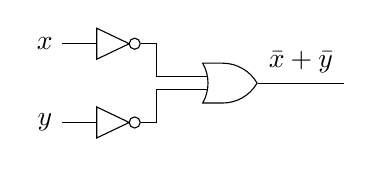
\begin{tikzpicture}[label distance=2mm]

        % INPUTS
        \node[] (x) at (0,1) {\normalsize $x$};
        \node[] (y) at (0,0) {\normalsize $y$};

        % NOTX
        \node[not gate US, draw] (NOTX) at ($(x) + (0.8, 0)$) {};
        \draw (x) -- (NOTX.input);

        % NOTY
        \node[not gate US, draw] (NOTY) at ($(y) + (0.8, 0)$) {};
        \draw (y) -- (NOTY.input);

        % XORY
        \node[or gate US, draw, rotate=0, logic gate inputs=nn] (XORY) at ($(NOTY) + (1.5, 0.5)$) {};
        \draw (NOTX.output) -- ([xshift=0.2cm]NOTX.output) |- (XORY.input 1);
        \draw (NOTY.output) -- ([xshift=0.2cm]NOTY.output) |- (XORY.input 2);
        \draw (XORY.output) -- node[above]{$\bar x + \bar y$} ($(XORY) + (1.5, 0)$);

    \end{tikzpicture}
}

\end{document} 
